\chapter{Problem Analysis}
\label{cha:Problem Analysis}
Lane merging is not a straightforward problem with a single solution. There are many different types of lane merging scenarios as well as a number of factors which add more variance to the problem. Section \ref{sec:Merge Types} analyses some of the different merging scenarios to better define them. Section \ref{sec:Measuring Success} indicates how success of a merge scheme can be measured and Section \ref{sec:Merge Variance Factors} defines some factors that could alter the behaviour of a given merge scenario.

\section{Merge Types}
\label{sec:Merge Types}
In this paper we focus on merges made at `critical positions' such as junctions. This is true for all of the merge scenarios analysed. Figure \ref{fig:laneCollection} illustrates some of the merge scenarios described.

\begin{figure}
\centerline{
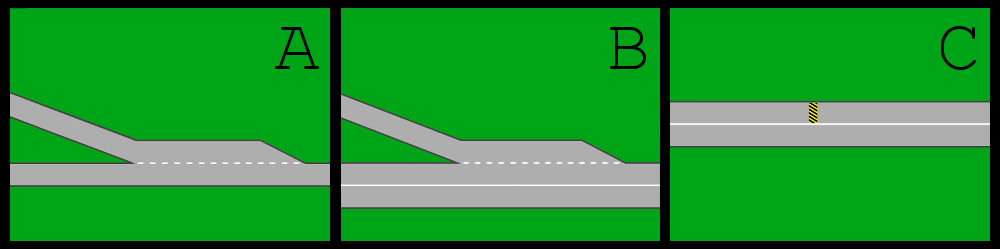
\includegraphics[width=14cm]{laneDiagrams/laneCollection.png}
}
\caption{a) S2S with slip lane, b) S2D with slip lane, c) Lane obstruction}
\label{fig:laneCollection}
\end{figure}

\subsection{Single-to-Single Merge}
\label{subsec:Single-to-Single Merge}
A single-to-single merge (S2S merge) describes a situation where a vehicle moves from a single lane road into another single lane road. In this situation we label the lane that vehicles are moving from, the `merge lane' (ML), and we label the lane that vehicles move to, the `target lane' (TL). The vehicles on the TL generally tend to be faster moving. We describe the vehicles that start on the ML as `merging vehicles' (MVs) and the vehicles that start on the TL as `TVs' (TVs). We have our critical position where the ML and TL intersect. We call this area the `merge zone'.

The main issue with an S2S merge stems from the limited options available to vehicles arriving at the critical position. Target vehicles do not have the opportunity to move laterally out of the way of MVs, and vehicles on both lanes could struggle to reduce their velocity without affecting their successors.

Many S2S merges are performed with an attached slip-road. A slip-road gives MVs more time to travel parallel to the TL before merging. This makes the merge easier for both MVs and TVs as MVs don't slow down in front of TVs in order to make the turn into the TL. Figure \ref{fig:laneCollection} A shows an S2S Merge with a slip lane.

\subsection{Single-to-Double Merge}
\label{subsec:Single-to-Double Merge}
A single-to-double merge (S2D merge) describes a situation where a vehicle moves from a single lane road into a double lane road. In this situation we have two TLs. The upper lane which directly links to the merging lane is called 'target lane 1' (TL1) and the lower lane is called 'target lane 2' (TL2). We still have only one critical position where the merging lane meets TL1.

An S2D merge provides more options for vehicles on the targets lanes at the critical position. Target vehicles now have the opportunity to move laterally to avoid MVs. Two lanes also allows for more vehicles on the TL which should give vehicles greater freedom to adjust their velocity without affecting their successors, at least when compared to the same number of vehicles on a single lane.

S2D merges can also take advantage of a slip-road. Figure \ref{fig:laneCollection} B shows an S2S Merge with a slip lane.

\subsection{Lane Obstruction Merge}
\label{subsec:Lane Obstruction Merge}
A lane obstruction merge is where a vehicle needs to change lanes to avoid an obstacle in their way. It is essentially an S2S merge although the vehicle moves laterally to avoid the obstacle. In this situation the critical position is a point shortly before the obstruction. 

The obstacle could be a broken down vehicle or some debris on the road. Because of the unexpected nature of the obstacle it may sometimes be difficult to have a centralised approach to the problem. Although, if the obstacle was a broken down vehicle, the vehicle might be able to act as the centralised system managing approaching vehicles. Figure \ref{fig:laneCollection} C shows an a lane obstruction merge scenario.

\section{Measuring Success}
\label{sec:Measuring Success}
In order to evaluate the effectiveness of solutions to the problems we need to define measurements of success. 

Solutions to the merging problems above must satisfy the following conditions:

\begin{enumerate}
\item \textit{No collisions}
This means avoiding collisions at the critical position between MVs and TVs, as well as avoiding collisions between vehicles on the same lane.
\item \textit{Minimise delays to both lanes}
Vehicles should not suffer large delays to travel time due to the merge. This means measuring average delay for both the ML and TL to ensure that the system is not starving one lane for the benefit of vehicles on the other.
\item \textit{Maximise throughput}
By minimising delays and velocity loss we aim to maximise the throughput of the critical position.
\item \textit{Minimise changes in velocity}
Though not strictly a performance requirement, the system should minimise changes in vehicle velocity, for both passenger comfort and vehicle efficiency.
\end{enumerate}

We need to measure how well solutions meet these conditions. 

\subsection{Collisions}
\label{subsec:Collisions}
Preventing collisions is a basic safety requirement for any autonomous vehicle system. We can measure this by comparing the positions of vehicles in the system, and ensuring that there is no overlap.

We should also consider measuring near misses. We can define a minimum spacing between vehicles, perhaps equal to the minimum braking distance of the vehicle plus an additional comfort distance. This would mimic the IDM model \citep{Treiber2000}.

Any collisions that do happen should be reported immediately. The system should automatically be considered a failure.

\subsection{Delay}
\label{subsec:Delay}
Delay measures the effect that the critical position had on the overall journey of the vehicle. It is the primary metric considered in Dresner et al.'s 2004 paper \citep{Dresner2004} on AIM.

Dresner et al. provide the following equation for measuring average delay.

\begin{equation}
\frac{1}{|C|}\sum_{v_i\in{C}}\bigl(t(i) - t_0(i)\bigr)
\end{equation}

$C$ is the set of vehicles that pass through a critical position within a set time frame. Assuming no other vehicles on the road, a vehicle $v_i$ would complete it's trip in time $t_0(i)$, otherwise $v_i$ would complete it's trip in time $t(i)$. We can represent this trip for vehicles in the simulator as the time difference between the vehicle spawning in and the vehicle being removed from the simulator.

To ensure fairness the mean delay will be measured across each lane.

\subsection{Throughput}
\label{subsec:Throughput}
By minimising delay we should also maximise throughput; the two are closely related. However we should also collect direct metrics.

\begin{equation}
\text{Vehicle throughput} = \frac{|C|}{t}
\end{equation}

Here $t$ is the time it took for all of the vehicles in $C$ to pass through the critical position. We will also need throughput measurements for each lane separately.

\subsection{Velocity Changes}
\label{subsec:Velocity Changes}
Vehicles should aim to reduce velocity changes as much as possible, particularly rapid changes. Ideally autonomous vehicles should have very smooth acceleration and braking profiles. This both increases passenger comfort and improves fuel efficiency. To measure maximum acceleration and deceleration we can measure the change in velocity at each time step in the simulator, and divide this change by the time-step length.

\section{Merge Variance Factors}
\label{sec:Merge Variance Factors}
In each of the scenarios in section \ref{sec:Merge Types} the road layout is fixed. More variance can be introduced to the scenarios by altering other factors. Not all of the factors below will be applicable in every merge scenario. Figure \ref{fig:s2sMarked} shows some of the factors below, applied to an S2S merge.

\begin{itemize}
\item \textit{Traffic Level} 
The traffic level changes the traffic density. It is measured in vehicles per hour per lane (\si{vhl})
\item \textit{Target lane speed limit}
The maximum speed that vehicles on the target lane can travel.
\item \textit{Merge lane speed limit}
The maximum speed that vehicles on the merge lane can travel.
\item \textit{Target lane lead in distance}
The distance between the point at which TVs arrive in the simulation and the point at which the TVs reach the merge zone.
\item \textit{Target lane lead out distance}
The distance between the end of the merge zone and the end of the target lane (at least the end in the simulator).
\item \textit{Merge lane lead in distance}
The distance between the point at which MVs arrive in the simulation and the point at which the MVs reach the merge zone.
\item \textit{Merging angle}
The interior angle $\theta$ at the point where the merging lane meets the target lane.
\item \textit{Slip-road length}
The length of the slip-road in a merge that uses a slip-road.
\end{itemize}

\begin{figure}[htb]
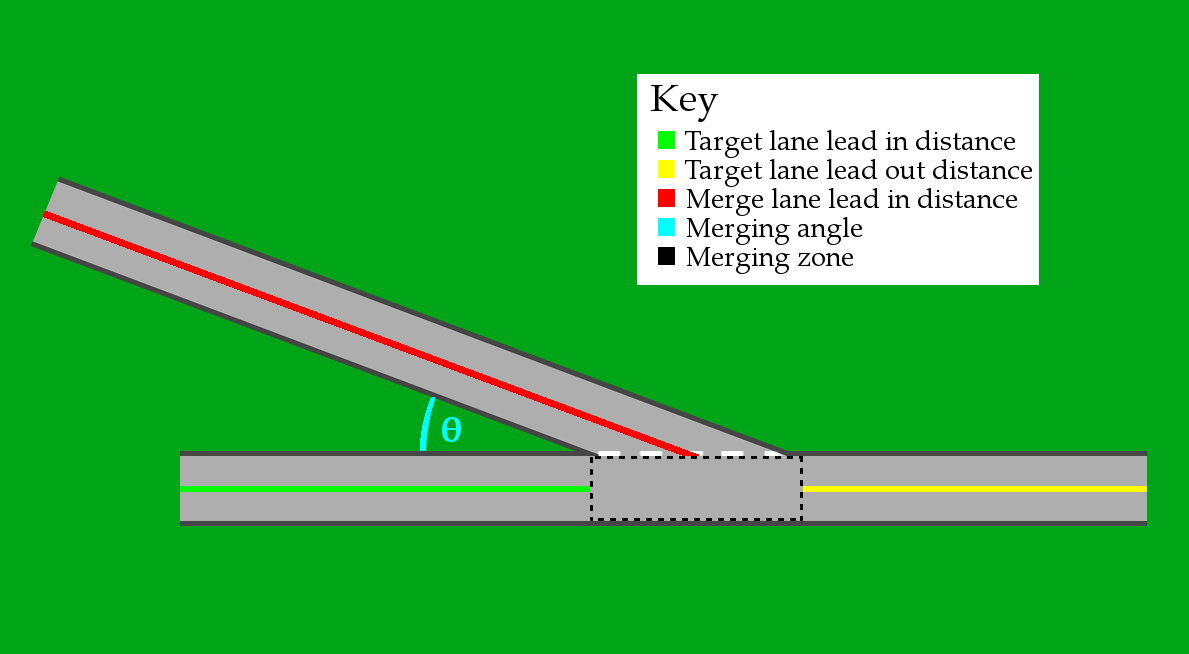
\includegraphics[width=\textwidth]{laneDiagrams/s2sMarked.png}
\caption{An S2S merge marked with some of the variance factors}
\label{fig:s2sMarked}
\end{figure}

Traffic level has a fairly obvious effect on performance in a particular merge scenario. The more vehicles that try to merge together the more difficult it will be for the merge to happen. It will likely require vehicles to move more slowly. Increased traffic density also increases the likelihood of traffic shocks, and vehicle manoeuvrability is impacted.

Altering speed limits could also affect performance. Higher speed limits could put pressure on systems that process the vehicles. Vastly differing speed limits for each lane could impact how easily a vehicle finds it to merge into another lane, and adapt to its speed limit.

Lead in distances change the amount of deliberation time vehicles have before they reach the junction. It also changes the distance they have to change their velocity in. This means that shorter distances could lead to larger acceleration and deceleration values as well as sub-optimal solutions to the merge. 

The merging angle changes the heading at which MVs arrive, but also the length of the merge zone. This could impact how long it takes a vehicle to traverse the merge zone as well as affecting how easily the vehicles adjust to the new lane heading.

\section{Requirements}
\label{sec:Requirements}
Using the problem analysis above, we can define requirements for our final system. This system will not deal with every merge scenario described but will instead set the groundwork for further research. The complete requirements are given in Appendix \ref{sec:RequirementsAppendix}. A shortened version with the most important requirements are given here.

\subsection{Functional Requirements}
\label{subsec:Functional Requirements}
The functional requirements describe the functionality required within the simulator. They are broken into two sets of requirements. User requirements and system requirements. User requirements describe the behaviour expected from the simulator from a user perspective. System requirements are all associated with a user requirement. They describe the functionality required by the system in order to satisfy the user requirement. Table \ref{tab:functionalRequirements} shows some of the functional requirements.

\begin{longtable}{|p{0.1\linewidth}|p{0.4\linewidth}|p{0.1\linewidth}|p{0.4\linewidth}|}
% Headings and Footers %
\caption{Functional requirements table.}\label{tab:functionalRequirements}\\
\hline
\multicolumn{2}{|l|}{User Requirements} & \multicolumn{2}{l|}{System Requirements} \\
\hline
\endfirsthead

\hline
\multicolumn{2}{|l|}{User Requirements} & \multicolumn{2}{l|}{System Requirements} \\
\hline
\endhead

\hline
\endfoot

\hline
\endlastfoot

% Data %

FU.3 & Users can run merge simulations. & FS.13 & The system can run merge simulations \\
\hline
FU.5 & User can view the activities of a simulation. & FS.51 & The system displays the current status of a simulation as it runs. \\
\hline
\multirow{2}{*}{FU.6} & \multirow{2}{*}{\parbox{\linewidth}{Users can export the results of a merge simulation.}}
 & FS.61 & The system has controls for exporting results data. \\
 &  & FS.62 & The system can produce a file containing results data from the simulation. \\
\hline
FU.7 & Users can select and run an S2S merge simulation. & FS.71 & The system can produce S2S simulations. \\
\hline
FU.8 & Users can select a centralised merging scheme with S2S merge simulations. & FS.81 & The system can use an AIM-like merge management system for the merging zone in an S2S simulation. \\
\hline
FU.9 & Users can select a decentralised merging scheme with S2S merge simulations & FS.91 & The system can use an merge management scheme similar to that described in \citetitle{VanMiddlesworth2008} \citep{VanMiddlesworth2008}. \\
\hline
FU.16 & Users should be alerted of any collisions during a simulation. & FS.161 & The system should be able to alert the user if a collision occurs. 
\end{longtable}

\subsection{Non-functional Requirements}
\label{subsec:Non-functional Requirements}
The non-functional requirements describe the expectations of the simulator that are not actions the simulator will perform. Table \ref{tab:nonFunctionalRequirements} shows some of the non-functional requirements for the simulator.

\begin{longtable}{|p{0.1\linewidth}|p{0.9\linewidth}|}
% Headings and footers %
\caption{Non-functional requirements table.}\label{tab:nonFunctionalRequirements}\\
\hline
ID & Description \\
\hline
\endfirsthead

\hline
ID & Description \\
\hline
\endhead

\hline
\endfoot

\hline
\endlastfoot

NS.6 & All data displayed to the user should be accurate. \\
\hline
NS.7 & All data in the results file should be accurate. \\
\hline
NS.9 & Code should be written to allow for easy expansion. \\
\hline
NS.11 & The simulator should be integrated into the AIM4 simulator without negatively affecting the performance of AIM simulations. \\
\end{longtable}